\section{PDF: Structure, Complexity, Vulnerabilities}
\label{sec:pdf}

\subsection{PDF Structure}

\begin{figure}[t]
    \centering
    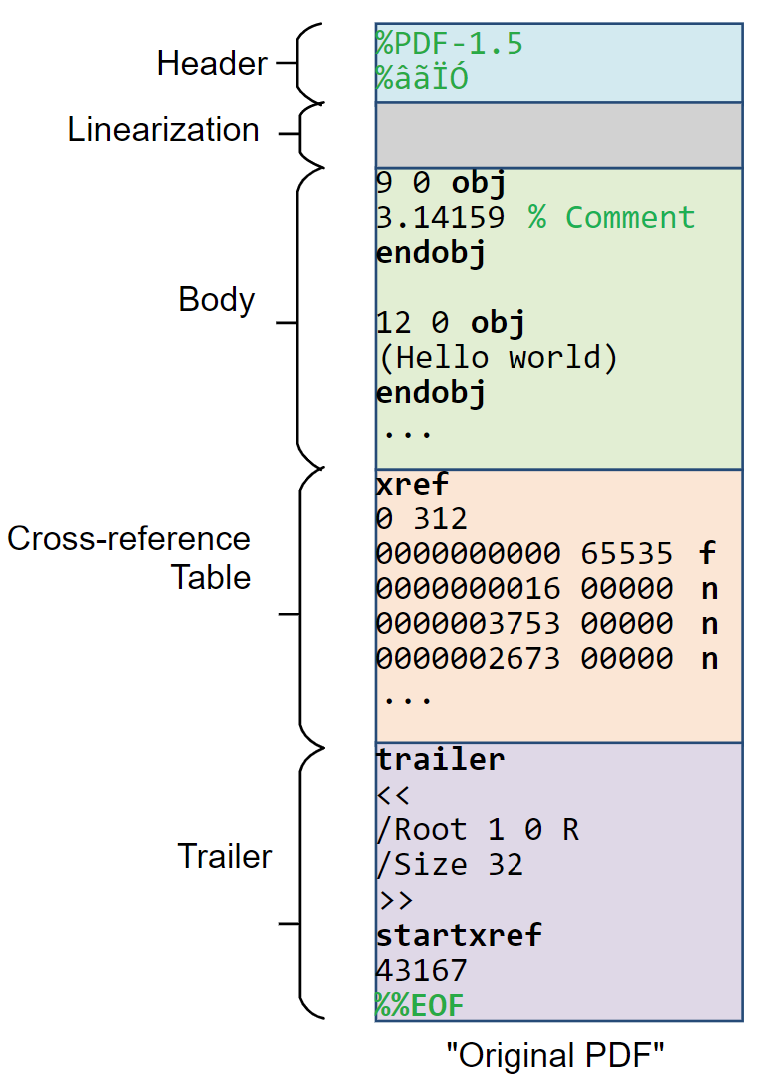
\includegraphics[width=0.65\linewidth]{figures/pdf-structure.png}
    \caption{PDF File Structure.}
    \label{fig:pdf-structure}
\end{figure}

PDF is a random-access file format that contains binary 8-bit data, line-based ASCII
text data (terminated with various end-of-line sequences), and a fixed format ASCII 
data format in different sections of a single file. The overall structure of a 
traditional PDF file without any incremental updates is shown in \cref{fig:pdf-structure} and 
described below, based on the official PDF Standard.
PDF 1.5 introduced more compact file structure capabilities known as cross-reference streams 
and object streams however since this builds on the following concepts, this modern 
variation on the PDF file structure will be described later.

The PDF \emph{Header} section contains the file identification marker as an ASCII
text comment line \lstcd{\%PDF-} followed by the PDF version as ASCII digits. 
An optional second comment line (starting with \lstcd{\%})
containing at least 4 bytes above 127 in value is recommended, as it ensures 
that PDF files are not misidentified as 7-bit text files. 
All file offsets in PDF file are from the \lstcd{\%} sign in \lstcd{\%PDF-x.y}.  

The \emph{Linearization} section is an optional optimization section that enables what is commonly
known as "fast web view". This section must occur within the first 1024 bytes of a PDF and contains
data that enables a Linearization-aware PDF processor to quickly display the opening page of a PDF
while the rest of a large PDF can download in the background.
Linearizatiom data is also invalidated by incremental updates (since an update might change objects
on the opening PDF page) and must therefore be checked and ignored.
As not all PDF parsers support Linearization, it is a known form of "parser differential by design". 
For the purposes of this paper, we will not consider Linearized PDF further.

The \emph{Body} section is where all indirect PDF objects are defined. Indirect PDF objects
are defined as those objects that have "a unique object identifier by which other objects can
refer to it (for example, as an element of an array or as the value of a dictionary entry)."
Any PDF object may be defined indirectly: integers, real numbers, strings, arrays, dictionaries, 
streams, etc. Objects are defined by their object identifier (their object number and generation 
number pair) followed by the keyword \lstcd{obj}. 
The end of every object is defined by the keyword \lstcd{endobj}.
In \cref{fig:pdf-structure}, object 9 is a real number (in ASCII) followed by a comment
(introduced by \lstcd{\%}) and this is followed by object 12 which is a PDF literal string object
(enclosed in \lstcd{(} and \lstcd{)}). The detailed syntax of PDF  
Every indirect object is reached by knowing the file offset to the start of the ASCII integer 
object number. This offset information for all indirect objects is stored in Cross-reference Tables.

The \emph{Cross-reference Table} section begins with the \lstcd{xref} keyword. For a PDF file
with no incremental updates, the next line will be a cross-reference sub-section text line comprising
two integers in ASCII (\lstcd{0 32} in this example). The first number is an object identifier 
and in the case of an original PDF this will always be 0. The second number is the number of
objects in the cross-reference section.
In traditional PDF each entry for an object contains a fixed length 20-byte line of text.
The first 10 ASCII digits represent the byte offset to the object, followed by a single ASCII SPACE, 
followed by 5 ASCII digits representing an object generation number. This is then followed by
another single ASCII space and the keyword \lstcd{n} for in-use objects or \lstcd{f} for free objects.
Finally the end-of-line sequence is defined to ensure that the entry for each objects has 
a 20-byte fixed length. A subtly is also that Cross-Reference sections are the only section in PDF where comments are expressly prohibited.


\todo{PW - incremental update description}
Each incremental update will normally append a Body, Cross-reference Table and Trailer sections to a PDF file with the entire original PDF remaining unchanged. The newly added incremental update trailer dictionary must also contain additional information referencing the immediately previous cross-reference table by byte offset. The Body of the incremental update will contain new objects, while the cross-reference table for the incremental update 

The \emph{Trailer} section is at the very end of every PDF file. 
It is defined as the end-of-file comment line \lstcd{\%\%EOF} immediately
preceded by the \lstcd{startxref} keyword followed by the file offset (decimal) to 
the cross-reference table in ASCII (i.e. the byte position of the \lstcd{xref} keyword 
from the the \lstcd{\%} of \lstcd{\%PDF-x.y}). Prior to this (but technically 
defined as being immediately \emph{after} the cross-reference table) is the trailer dictionary
identified by just the \lstcd{trailer} keyword, rather than the \lstcd{obj} and \lstcd{endobj}
keywords used in the PDF Body section.

The above paragraphs describe the physical layout of a PDF, but the processing sequence may not be so apparent. The following paragraphs walk through the processing necessary to correctly parse a PDF file with incremental updates.

PDF parsing begins by locating the PDF Header as it is not uncommon for PDF files to have 
preamble bytes (such as HTTP header or HTML fragment). Thus the zero-offset byte is 
determined from the \lstcd{\%} sign in \lstcd{\%PDF-x.y}. Processing then continues by
seeking to end-of-file and locating the end-of-file marker \lstcd{\%\%EOF}.

\todo{PW - restart here}

... and then locate either the \lstcd{xref} keyword for
traditional PDF cross-reference tables, or a PDF object that should be
a cross-reference stream.  In the case of traditional PDF
cross-reference tables, after the cross reference table will be the
trailer dictionary identified by the \lstcd{trailer} keyword or,
alternatively for PDF 1.5 and later files with cross-reference
streams, the trailer dictionary keys will be in the stream extent
dictionary of the cross reference stream.

... these are identified by a \lstcd{Prev} entry in either the trailer
dictionary or the stream extent dictionary of a cross-reference stream. The
value of the \lstcd{Prev} key is another byte offset to the immediately
preceding incremental update which, again, can either be a traditional
cross-reference table and to the start of the \lstcd{xref} keyword, or to a
cross-reference stream. This process repeats, working from the most recent
update back through time to the original PDF document.

Of particular note is the \lstcd{Size} entry, which
is one greater than the largest object number allocated in the PDF
file.

In this stage, data in each cross reference table must then be parsed to
identify the byte offset to the start of each PDF object. Note also that PDF
does not define the byte offset to the end of an object.

There are two sets of
objects in every PDF document: the in-use list of PDF objects and a free list
of PDF objects. Object zero is always the start of the free list as it is not
otherwise a valid object number.

For incremental updates, PDF object numbering
does not have to be sequential, with skipped object numbers assumed to be on
the free list (although this is not stated explicitly in the PDF
specification).

Parsing depends on the form of the incremental update, with
traditional cross-reference tables being simpler and largely independent of
other processing. Cross-reference streams however are more complex as they are
usually compressed and thus require the pre-DOM parser to "trust" the stream
extent dictionary data.

Each incremental update can add new objects, mark existing in-use objects as
free, or reinstate previously freed objects.


\mttodo{maybe: import the type definitions}

\subsection{Root Causes of PDF Complexity}

Most data formats can be described by much simpler mechanisms;
most language processors (e.g., a Python parser) can be described and parsed by
textbook methods (e.g., the old \emph{lex} and \emph{yacc} are sufficient for
most language processors);
so what makes PDF processing so much more complex?
\begin{lstlisting}[style=meta]
  - indirect offsets
    - which may recursively point to other indirect offsets
    - need programming language
      (or a 'seek' in the data definition lang)
  - DOM is a directed graph structure that allows cycles and arbitrary references (so not a DAG)
    - objects point to objects via byte offsets (cf. not by nested expressions such as XML)  
  - backwards parsing
  - incremental updates as a set of deltas to be applied to the file, which change the DOM
    - (note: unlike HTML, PDF's DOM is fixed and cannot be altered by JS)
  - XRef tables ...
  - ... giving rise to cavities
    - giving rise to polyglots
  - dependent parsers
\end{lstlisting}

\subsection{\todo{para. needs home: ``data integrity relationships...''}}

\todo{we should use the concept of "data integrity relationships" being the
  essence of the necessary context. e.g. PDF incremental updates are appended to
  a previously valid PDF - thus an incremental update should not "make visible"
  a PDF object that was not already valid and visible in the original PDF (this
  is one method Shadow Attacks use - cf. an upstream "supply chain attack" by an
  attacker), even if that PDF object is otherwise entirely syntactically
  valid. In the same way an incremental update that refers to an object at a
  file byte offset after the incremental update would be highly suspicious.}

% ------------------------------------------------------------------------------
\subsection{Vulnerabilities \note{1pp}}
\label{sec:vulnerabilities}

% As will become even more apparent, there is a significant amount of
% parsing and computation that needs to be done \emph{pre-DOM}.

Given our recent points about the \emph{PDF Trust Chain}
(\cref{sec:trust-chain}),
it should not surprise us that most of the PDF attack vectors
involve some aspect of breaking the \emph{DOM} abstraction.
I.e., the vulnerabilities occur \emph{pre-DOM}.

{\bf{Shadow Attacks}} \todo{...}

{\bf{Schizophrenia}} \todo{should define what we mean by schizo - is this the same thing that gives rise to parser differentials or a feature of of the syntax or layout of PDF?}
\begin{lstlisting}[style=meta]
  - writer errors
  - parser differentials
    - e.g., ignoring XRef tables
  - recovering parsers !!
  - blind faith in incremental updates (Shadow Attacks)
\end{lstlisting}

{\bf{Polyglots}} 
\todo{... arising from cavities and permissive implementations and ...}
\begin{lstlisting}[style=meta]
- Multiple places for hidden/unused/malicious data in PDF
  - non-obvious places, unnoticed when "simply parsing"
  - e.g., shadow-attacks
  - dead bytes, dead objects, dead updates, dead linearization sections, etc.
\end{lstlisting}

{\bf{Denial of Service (DOS)}} 
%
\begin{lstlisting}[style=meta]
- [potential recursion many places]
- format may not be well-defined because the recursion is not
    "well-defined"
\end{lstlisting}



{\bf{Others}} \todo{Maybe PII/redaction issues - just 'cos you delete something in a PDF doesn't mean it is really deleted (thanks to incremental updates)!!!! }

